\section{Pilot Study}
\label{sec:pilot}

Our pilot study uses CRIT, and it aims to answer two questions:
Should all prompts be issued to GPT-3 sequentially or they
can be issued all together?  
What limitations can be identified for improvement?
The study utilizes exercises with established answers from the $8^{th}$ edition of the textbook ``Ask the Right Questions'' by the authors of \cite{AskRightQ2001}. It is important to note that the study evaluates the effectiveness of CRIT's prompt template, rather than the language models to which CRIT can issue prompts.


\vspace{.1in}
\noindent
{\bf Example Article} (\cite{AskRightQ2001}, p23.)
\noindent
\begin{table}[h!]
\vspace{-.1in}
\normalsize
\begin{tabular}{p{8.4cm}}
{\em Television advertising agencies are very clever in the way that they construct ads. Often the ads are similar to the cartoons that the children enjoy. Children see these characters interacting with a certain product and associate their affection for the character with affection for the product. The companies do not want the children to perceive a difference between the shows they are watching and the advertisements. By using this strategy, these companies take advantage of the fact that children are often not able to discriminate between the cartoons and the ads and do not understand that these things offered come at a cost. Often the advertising is about sugary snacks or fatty foods, leading the children down a path to bad health. Advertising geared towards children should be regulated, just as there are regulations now about tobacco and alcohol ads targeted at children.}
\end{tabular}
\end{table}

On short documents, the results are similar in quality when CRIT is used to issue prompts either sequentially or all together as one prompt, as long as the instructions are consistent. However, when evaluating long articles in \cite{501Q2004}, CRIT issuing prompts one after another yields much higher presentation quality in both organization and clarity. 
(Due to the space limit, we document long-document
evaluation in a supplement document \cite{CRITExtended2023}.) In the teaching mode, the sequential option is thus much preferred. Furthermore,
When a reason is itself a claim and requires CRIT to validate its supporting references, using a sequential approach is more flexible and enables CRIT to query for references and then execute the process recursively.


\begin{table}[t!]
%\vspace{-.05in}
%\resizebox{\textwidth}{!}
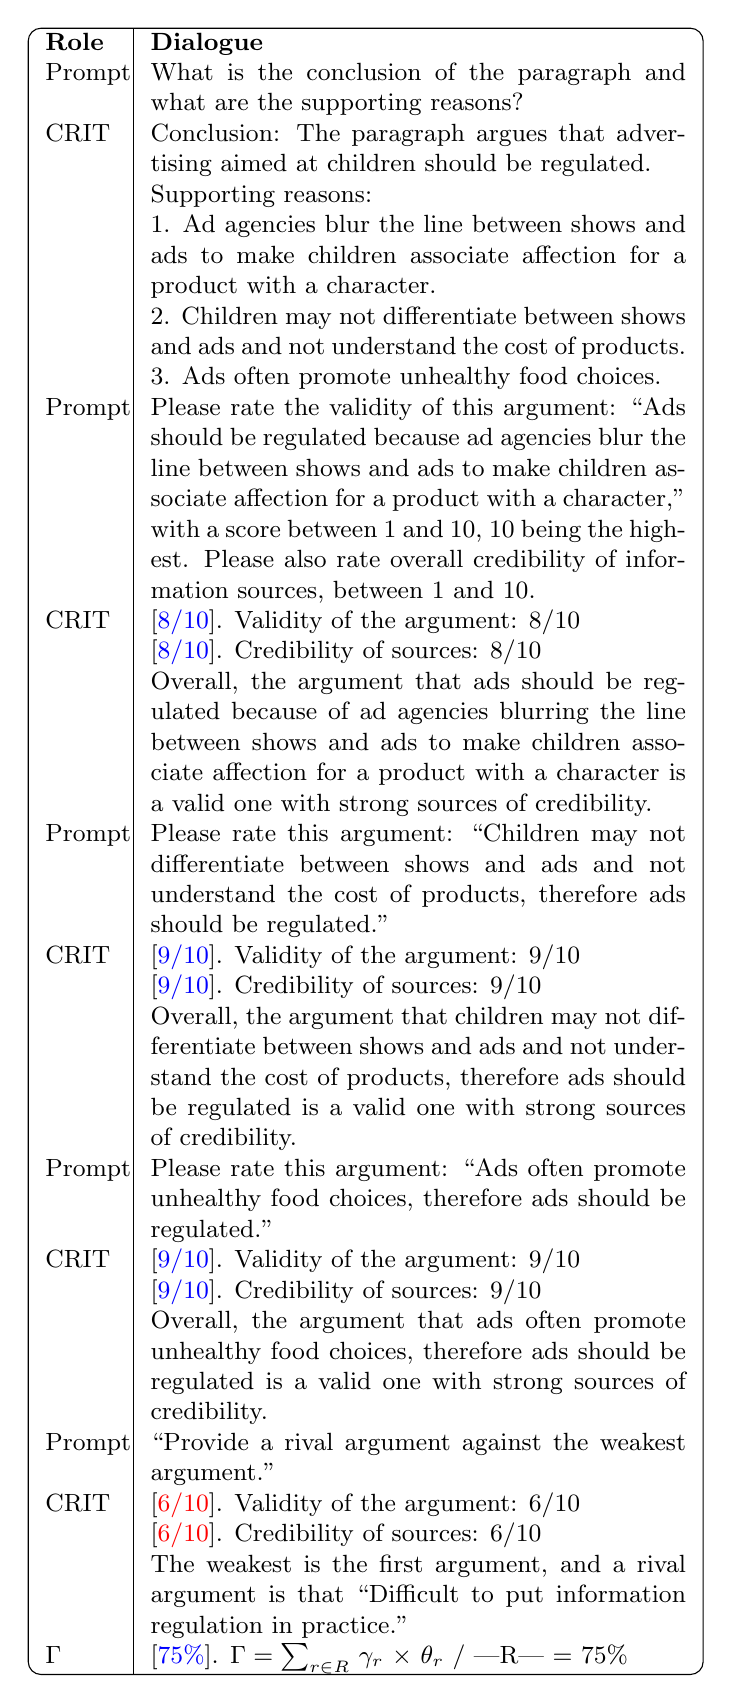
\begin{tikzpicture}
\begin{small}
\node (table) [inner sep=0pt] {
\begin{tabular}{p{0.9cm}|p{6.8cm}}
\toprule
\textbf{Role} & \textbf{Dialogue} \\
\midrule
Prompt & {What is the conclusion of the paragraph and what are the supporting reasons?} \\
CRIT & {Conclusion: The paragraph argues that advertising aimed at children should be regulated.

Supporting reasons:

1. Ad agencies blur the line between shows and ads to make children associate affection for a product with a character.

2. Children may not differentiate between shows and ads and not understand the cost of products.

3. Ads often promote unhealthy food choices.
} \\

\midrule
Prompt & {Please rate the validity of this argument: ``Ads should be regulated because ad agencies blur the line between shows and ads to make
children associate affection for a product with a character," with a score between 1 and 10, 10 being the highest. Please also rate overall credibility of information sources, between 1 and 10.} \\
CRIT & {
[{\color{blue}8/10}]. Validity of the argument: 8/10

[{\color{blue}8/10}]. Credibility of sources: 8/10

Overall, the argument that ads should be regulated because of ad agencies blurring the line between shows and ads to make children associate affection for a product with a character is a valid one with strong sources of credibility.} \\

Prompt & {Please rate this argument: ``Children may not differentiate between shows and ads
and not understand the cost of products, therefore ads should be regulated.''} \\

CRIT &
{[{\color{blue}9/10}]. Validity of the argument: 9/10

[{\color{blue}9/10}]. Credibility of sources: 9/10

Overall, the argument that children may not differentiate between shows and ads and not understand the cost of products, therefore ads should be regulated is a valid one with strong sources of credibility.} \\

Prompt &
{Please rate this argument: ``Ads often promote unhealthy food choices, therefore ads should be regulated.''} \\

CRIT &
{[{\color{blue}9/10}]. Validity of the argument: 9/10

[{\color{blue}9/10}]. Credibility of sources: 9/10

Overall, the argument that ads often promote unhealthy food choices, therefore ads should be regulated is a valid one with strong sources of credibility.
} \\
Prompt &
{``Provide a rival argument against the weakest argument.''} \\

\midrule
CRIT & {
{[{\color{red}6/10}]. Validity of the argument: 6/10

[{\color{red}6/10}]. Credibility of sources: 6/10

The weakest is the first argument, and a rival argument is that ``Difficult to put information regulation in practice.''} 
} \\
\midrule
%\vspace{.1cm}
{$\Gamma$} & [{\color{blue}$75\%$}]. $\Gamma = \sum_{r \in R}$
\text{${\gamma}_r$ $\times$ \text{${\theta}_r$} / |R| 
= $75\%$} \\
%\vspace{.1cm}
%\bottomrule
\end{tabular}
};
\draw [rounded corners=.5em] (table.north west) rectangle (table.south east);
\end{small}
\end{tikzpicture}
%\vspace{.01in}
\caption{Pilot Study.}
\label{tab:Validation}
\vspace{-.2in}
\end{table}

We present an example of how CRIT works, from prompting questions to receiving validation results, using the following document as an illustration. In Table~\ref{tab:Validation}, we show both the claim and the supporting reasons to the claim extracted by GPT-3. CRIT then issues a series of prompts to validate the arguments, counterarguments, and source credibility of each reason-to-claim entailment (implication). 

The second segment of Table~\ref{tab:Validation} displays the validation dialogue between CRIT and GPT-3. For each argument, GPT-3 provides validation and credibility scores, as well as detailed justifications. 
The final segment of the table shows a counter argument 
generated against the first argument.
Since GPT-3 evaluates the counterargument being ``difficult to put information regulation in practice'' and rates it $0.6 \times 0.6$, it was dismissed due to low validity. 
The final aggregated score is $\Lambda = 75\%$,
which is considered high.


%The negative score of the rival argument
%is $0.6 \times 0.6 = 0.36$, which is considered low.
%(Due to space limitations, the table only includes GPT-3's summary for each argument.)